% Created by tikzDevice version 0.10.1 on 2018-01-23 02:20:17
% !TEX encoding = UTF-8 Unicode
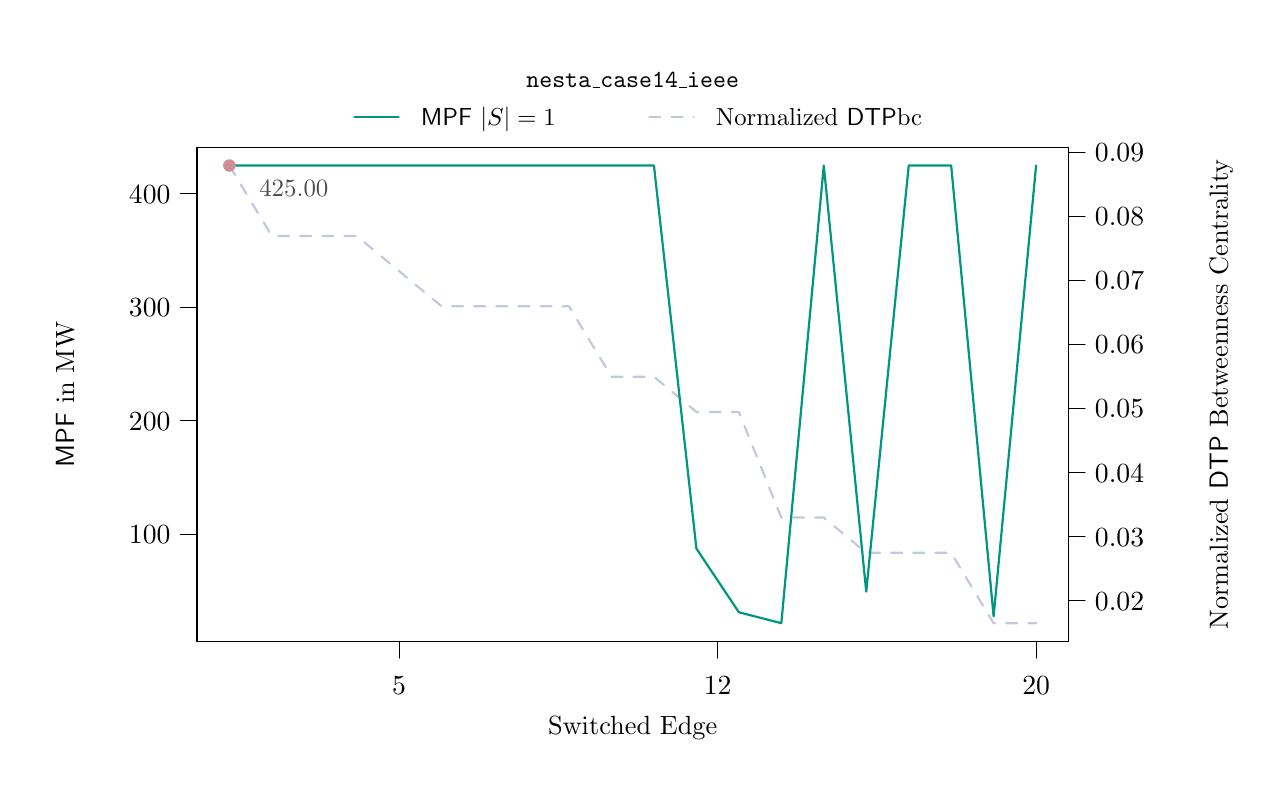
\begin{tikzpicture}[x=1pt,y=1pt]
\definecolor{fillColor}{RGB}{255,255,255}
\path[use as bounding box,fill=fillColor,fill opacity=0.00] (0,0) rectangle (440.85,271.01);
\begin{scope}
\path[clip] (  0.00,  0.00) rectangle (440.85,271.01);
\definecolor{drawColor}{RGB}{193,202,220}

\path[draw=drawColor,line width= 0.8pt,dash pattern=on 4pt off 4pt ,line join=round,line cap=round] ( 72.86,221.20) --
	( 88.20,195.75) --
	(103.55,195.75) --
	(118.89,195.75) --
	(134.23,183.03) --
	(149.58,170.31) --
	(164.92,170.31) --
	(180.26,170.31) --
	(195.61,170.31) --
	(210.95,144.87) --
	(226.30,144.87) --
	(241.64,132.15) --
	(256.98,132.15) --
	(272.33, 93.98) --
	(287.67, 93.98) --
	(303.01, 81.26) --
	(318.36, 81.26) --
	(333.70, 81.26) --
	(349.04, 55.82) --
	(364.39, 55.82);
\end{scope}
\begin{scope}
\path[clip] (  0.00,  0.00) rectangle (440.85,271.01);
\definecolor{drawColor}{RGB}{0,0,0}

\path[draw=drawColor,line width= 0.4pt,line join=round,line cap=round] ( 61.20, 49.20) --
	(376.05, 49.20) --
	(376.05,227.81) --
	( 61.20,227.81) --
	( 61.20, 49.20);
\end{scope}
\begin{scope}
\path[clip] (  0.00,  0.00) rectangle (440.85,271.01);
\definecolor{drawColor}{RGB}{0,0,0}

\path[draw=drawColor,line width= 0.4pt,line join=round,line cap=round] (376.05, 63.96) -- (376.05,226.03);

\path[draw=drawColor,line width= 0.4pt,line join=round,line cap=round] (376.05, 63.96) -- (382.05, 63.96);

\path[draw=drawColor,line width= 0.4pt,line join=round,line cap=round] (376.05, 87.11) -- (382.05, 87.11);

\path[draw=drawColor,line width= 0.4pt,line join=round,line cap=round] (376.05,110.26) -- (382.05,110.26);

\path[draw=drawColor,line width= 0.4pt,line join=round,line cap=round] (376.05,133.42) -- (382.05,133.42);

\path[draw=drawColor,line width= 0.4pt,line join=round,line cap=round] (376.05,156.57) -- (382.05,156.57);

\path[draw=drawColor,line width= 0.4pt,line join=round,line cap=round] (376.05,179.72) -- (382.05,179.72);

\path[draw=drawColor,line width= 0.4pt,line join=round,line cap=round] (376.05,202.88) -- (382.05,202.88);

\path[draw=drawColor,line width= 0.4pt,line join=round,line cap=round] (376.05,226.03) -- (382.05,226.03);

\node[text=drawColor,anchor=base west,inner sep=0pt, outer sep=0pt, scale=  1.00] at (385.65, 60.51) {0.02};

\node[text=drawColor,anchor=base west,inner sep=0pt, outer sep=0pt, scale=  1.00] at (385.65, 83.67) {0.03};

\node[text=drawColor,anchor=base west,inner sep=0pt, outer sep=0pt, scale=  1.00] at (385.65,106.82) {0.04};

\node[text=drawColor,anchor=base west,inner sep=0pt, outer sep=0pt, scale=  1.00] at (385.65,129.97) {0.05};

\node[text=drawColor,anchor=base west,inner sep=0pt, outer sep=0pt, scale=  1.00] at (385.65,153.13) {0.06};

\node[text=drawColor,anchor=base west,inner sep=0pt, outer sep=0pt, scale=  1.00] at (385.65,176.28) {0.07};

\node[text=drawColor,anchor=base west,inner sep=0pt, outer sep=0pt, scale=  1.00] at (385.65,199.43) {0.08};

\node[text=drawColor,anchor=base west,inner sep=0pt, outer sep=0pt, scale=  1.00] at (385.65,222.59) {0.09};
\end{scope}
\begin{scope}
\path[clip] (  0.00,  0.00) rectangle (440.85,271.01);
\definecolor{drawColor}{RGB}{0,150,130}

\path[draw=drawColor,line width= 0.8pt,line join=round,line cap=round] ( 72.86,221.20) --
	( 88.20,221.20) --
	(103.55,221.20) --
	(118.89,221.20) --
	(134.23,221.20) --
	(149.58,221.20) --
	(164.92,221.20) --
	(180.26,221.20) --
	(195.61,221.20) --
	(210.95,221.20) --
	(226.30,221.20) --
	(241.64, 82.80) --
	(256.98, 59.77) --
	(272.33, 55.82) --
	(287.67,221.20) --
	(303.01, 67.23) --
	(318.36,221.20) --
	(333.70,221.20) --
	(349.04, 58.28) --
	(364.39,221.20);
\end{scope}
\begin{scope}
\path[clip] (  0.00,  0.00) rectangle (440.85,271.01);
\definecolor{drawColor}{RGB}{0,0,0}

\path[draw=drawColor,line width= 0.4pt,line join=round,line cap=round] ( 61.20, 49.20) --
	(376.05, 49.20) --
	(376.05,227.81) --
	( 61.20,227.81) --
	( 61.20, 49.20);
\end{scope}
\begin{scope}
\path[clip] (  0.00,  0.00) rectangle (440.85,271.01);
\definecolor{drawColor}{RGB}{0,0,0}

\path[draw=drawColor,line width= 0.4pt,line join=round,line cap=round] ( 61.20, 87.92) -- ( 61.20,210.95);

\path[draw=drawColor,line width= 0.4pt,line join=round,line cap=round] ( 61.20, 87.92) -- ( 55.20, 87.92);

\path[draw=drawColor,line width= 0.4pt,line join=round,line cap=round] ( 61.20,128.93) -- ( 55.20,128.93);

\path[draw=drawColor,line width= 0.4pt,line join=round,line cap=round] ( 61.20,169.94) -- ( 55.20,169.94);

\path[draw=drawColor,line width= 0.4pt,line join=round,line cap=round] ( 61.20,210.95) -- ( 55.20,210.95);

\node[text=drawColor,anchor=base east,inner sep=0pt, outer sep=0pt, scale=  1.00] at ( 51.60, 84.48) {100};

\node[text=drawColor,anchor=base east,inner sep=0pt, outer sep=0pt, scale=  1.00] at ( 51.60,125.49) {200};

\node[text=drawColor,anchor=base east,inner sep=0pt, outer sep=0pt, scale=  1.00] at ( 51.60,166.49) {300};

\node[text=drawColor,anchor=base east,inner sep=0pt, outer sep=0pt, scale=  1.00] at ( 51.60,207.50) {400};
\end{scope}
\begin{scope}
\path[clip] (  0.00,  0.00) rectangle (440.85,271.01);
\definecolor{fillColor}{RGB}{207,142,147}

\path[fill=fillColor] ( 72.86,221.20) circle (  2.25);
\end{scope}
\begin{scope}
\path[clip] (  0.00,  0.00) rectangle (440.85,271.01);
\definecolor{drawColor}{RGB}{0,0,0}

\path[draw=drawColor,line width= 0.4pt,line join=round,line cap=round] ( 61.20, 49.20) --
	(376.05, 49.20) --
	(376.05,227.81) --
	( 61.20,227.81) --
	( 61.20, 49.20);
\end{scope}
\begin{scope}
\path[clip] (  0.00,  0.00) rectangle (440.85,271.01);
\definecolor{drawColor}{gray}{0.30}

\node[text=drawColor,anchor=base,inner sep=0pt, outer sep=0pt, scale=  0.90] at ( 96.18,210.04) {425.00};
\end{scope}
\begin{scope}
\path[clip] (  0.00,  0.00) rectangle (440.85,271.01);
\definecolor{drawColor}{RGB}{0,0,0}

\path[draw=drawColor,line width= 0.4pt,line join=round,line cap=round] (134.23, 49.20) -- (364.39, 49.20);

\path[draw=drawColor,line width= 0.4pt,line join=round,line cap=round] (134.23, 49.20) -- (134.23, 43.20);

\path[draw=drawColor,line width= 0.4pt,line join=round,line cap=round] (249.31, 49.20) -- (249.31, 43.20);

\path[draw=drawColor,line width= 0.4pt,line join=round,line cap=round] (364.39, 49.20) -- (364.39, 43.20);

\node[text=drawColor,anchor=base,inner sep=0pt, outer sep=0pt, scale=  1.00] at (134.23, 30.00) {5};

\node[text=drawColor,anchor=base,inner sep=0pt, outer sep=0pt, scale=  1.00] at (249.31, 30.00) {12};

\node[text=drawColor,anchor=base,inner sep=0pt, outer sep=0pt, scale=  1.00] at (364.39, 30.00) {20};

\node[text=drawColor,anchor=base,inner sep=0pt, outer sep=0pt, scale=  0.95] at (218.62, 15.60) {Switched Edge};

\node[text=drawColor,rotate= 90.00,anchor=base,inner sep=0pt, outer sep=0pt, scale=  0.95] at ( 16.80,138.51) {$\mathsf{MPF}$ in~$\mathrm{MW}$};

\node[text=drawColor,rotate= 90.00,anchor=base,inner sep=0pt, outer sep=0pt, scale=  0.95] at (433.65,138.51) {Normalized~$\mathsf{DTP}$ Betweenness Centrality};
\end{scope}
\begin{scope}
\path[clip] (  0.00,  0.00) rectangle (440.85,271.01);
\definecolor{drawColor}{RGB}{0,150,130}

\path[draw=drawColor,line width= 0.8pt,line join=round,line cap=round] (118.04,238.60) -- (134.06,238.60);
\definecolor{drawColor}{RGB}{193,202,220}

\path[draw=drawColor,line width= 0.8pt,dash pattern=on 4pt off 4pt ,line join=round,line cap=round] (224.63,238.60) -- (240.65,238.60);
\definecolor{drawColor}{RGB}{0,0,0}

\node[text=drawColor,anchor=base,inner sep=0pt, outer sep=0pt, scale=  0.89] at (218.62,249.28) {\texttt{nesta\_case14\_ieee}};

\node[text=drawColor,anchor=base west,inner sep=0pt, outer sep=0pt, scale=  0.89] at (142.07,235.54) {$\mathsf{MPF}~|S|=1$};

\node[text=drawColor,anchor=base west,inner sep=0pt, outer sep=0pt, scale=  0.89] at (248.66,235.54) {Normalized~$\mathsf{DTP}$bc};
\end{scope}
\end{tikzpicture}
